% =====================================================================
%  StoryLens — Slide thuyết trình cuối kỳ (PA5)
%  CSC10011 · Công nghệ phần mềm cho hệ thống Trí tuệ Nhân tạo · HCMUS
%
%  Biên dịch:  xelatex StoryLens_Slides.tex   (chạy 2 lần)
%  Yêu cầu:    XeLaTeX + beamer + tcolorbox + tikz ; font hệ thống Arial/Calibri
%
%  Thiết kế "manga-editorial" đồng bộ với sản phẩm:
%  góc vuông sắc, viền đậm, bóng cứng lệch (panel-shadow),
%  nhãn chữ hoa giãn ký tự, tông mực đen + đỏ manga + vàng nhấn.
% =====================================================================
\documentclass[aspectratio=169,10pt]{beamer}

\usepackage{fontspec}
\usepackage{xcolor}
\usepackage[most]{tcolorbox}
\tcbuselibrary{skins,raster}
\usepackage{tikz}
\usepackage{graphicx}
\usepackage{colortbl}
\usepackage{array}
\usepackage{amssymb}
\usetikzlibrary{calc,shapes.geometric}

% ---------- Bảng màu ----------
\definecolor{ink}{HTML}{191512}
\definecolor{ink2}{HTML}{3A332C}
\definecolor{paper}{HTML}{FFFFFF}
\definecolor{cream}{HTML}{F4EEE3}
\definecolor{mred}{HTML}{D0311E}
\definecolor{gold}{HTML}{E0A32E}
\definecolor{mblue}{HTML}{285B7A}
\definecolor{mgreen}{HTML}{2E7D4F}
\definecolor{slate}{HTML}{6E665D}
\definecolor{hair}{HTML}{D8D0C4}
\definecolor{softwhite}{HTML}{C9C0B4}

% ---------- Font (hệ thống Windows, hỗ trợ tiếng Việt) ----------
\setsansfont{Arial}
\setmainfont{Calibri}
\newfontfamily\headfont{Arial}
\renewcommand{\familydefault}{\sfdefault}

% ---------- Beamer cơ bản ----------
\setbeamertemplate{navigation symbols}{}
\setbeamercolor{background canvas}{bg=paper}
\setbeamercolor{normal text}{fg=ink}
\setbeamercolor{itemize item}{fg=mred}
\setbeamercolor{itemize subitem}{fg=slate}
\setbeamertemplate{itemize item}{\footnotesize\raise0.2ex\hbox{\textbullet}}
\setbeamerfont{itemize/enumerate body}{size=\small}
\setlength{\parindent}{0pt}

% ---------- Chân trang (số trang / 26) ----------
\setbeamertemplate{footline}{%
  \hbox{%
  \begin{beamercolorbox}[wd=\paperwidth,ht=3ex,dp=1.4ex,leftskip=0.55cm,rightskip=0.55cm]{}%
   {\footnotesize\headfont\bfseries\textcolor{ink}{StoryLens}%
    \textcolor{slate}{\ \ $\cdot$\ Nhóm 1 $\cdot$ CSC10011}}\hfill
   {\footnotesize\textcolor{slate}{\insertframenumber\,/\,28}}%
  \end{beamercolorbox}}%
}

% ---------- Kiểu thẻ (panel bóng cứng lệch) ----------
\tcbset{
  card/.style={enhanced, sharp corners, boxrule=1pt, colframe=ink, colback=white,
    shadow={0.6mm}{-0.6mm}{0mm}{fill=ink},
    fonttitle=\headfont\bfseries, left=2mm, right=2mm, top=1.4mm, bottom=1.4mm},
  darkcard/.style={enhanced, sharp corners, boxrule=1pt, colframe=ink, colback=ink, coltext=white,
    shadow={0.6mm}{-0.6mm}{0mm}{fill=mred},
    fonttitle=\headfont\bfseries\color{gold}, left=2.5mm, right=2.5mm, top=2mm, bottom=2mm},
  creamcard/.style={enhanced, sharp corners, boxrule=1pt, colframe=ink, colback=cream,
    shadow={0.6mm}{-0.6mm}{0mm}{fill=ink},
    fonttitle=\headfont\bfseries, left=2mm, right=2mm, top=1.4mm, bottom=1.4mm},
}

% ---------- Lệnh tiện ích ----------
\newcommand{\kick}[1]{{\headfont\bfseries\footnotesize\textcolor{mred}{\MakeUppercase{#1}}}}
\newcommand{\kickg}[1]{{\headfont\bfseries\footnotesize\textcolor{gold}{\MakeUppercase{#1}}}}
\newcommand{\slidehead}[2]{%
  \kick{#1}\par\vspace{0.6mm}%
  {\headfont\bfseries\LARGE\textcolor{ink}{#2}}\par\vspace{1.2mm}}
\newcommand{\arr}{\textcolor{mred}{\,\raisebox{0.1ex}{$\rightarrow$}\,}}
% Huy hiệu số vuông
\newcommand{\numbadge}[2][ink]{\tikz[baseline=-0.5ex]{\fill[#1] (0,-0.28) rectangle (0.56,0.28);
  \node[white,font=\headfont\bfseries] at (0.28,0){#2};}}

% =====================================================================
\begin{document}

% ---------------------------------------------------------------------
% SLIDE 1 — TITLE (dark, plain)
% ---------------------------------------------------------------------
{\setbeamercolor{background canvas}{bg=ink}
\begin{frame}[plain]
\begin{tikzpicture}[remember picture,overlay]
  % thanh dọc đỏ
  \fill[mred] (current page.north west) rectangle ++(0.22,-\paperheight);
  % ô vàng + chip logo trường HCMUS (nền trắng, bóng đỏ)
  \fill[gold] ($(current page.north east)+(-2.35,-0.55)$) rectangle ++(0.42,-0.42);
  \fill[mred] ($(current page.north east)+(-1.78,-0.7)$) rectangle ++(1.4,-1.4);
  \fill[white] ($(current page.north east)+(-1.88,-0.6)$) rectangle ++(1.4,-1.4);
  \node[anchor=north east,inner sep=0] at ($(current page.north east)+(-0.6,-0.72)$)
     {
\includegraphics[width=1.16cm]{assets/hcmus_logo.png}};
\end{tikzpicture}
\vspace{0.7cm}
\hspace{0.7cm}\begin{minipage}{0.86\paperwidth}
  \kickg{Báo cáo đồ án cuối kỳ · PA5}\par\vspace{2mm}
  {\headfont\bfseries\fontsize{56}{60}\selectfont\textcolor{white}{StoryLens}}\par\vspace{2.5mm}
  {\color{mred}\rule{9.2cm}{1.6pt}}\par\vspace{2mm}
  {\headfont\Large\textcolor{white}{Nền tảng AI dịch \& hỏi–đáp Manga theo ngữ cảnh}}\par\vspace{1.5mm}
  {\small\textcolor{softwhite}{Upload \arr\ phát hiện · đọc · xoá nền · dịch bong bóng thoại (Nhật/Trung \arr\ Việt) \arr\ đọc overlay + RAG Q\&A}}\par\vspace{7mm}
  \footnotesize
  \begin{tabular}{@{}p{3.35cm}p{3.35cm}p{3.35cm}p{3.35cm}@{}}
    {\color{gold}\headfont\bfseries MÔN HỌC} & {\color{gold}\headfont\bfseries GVHD} & {\color{gold}\headfont\bfseries NHÓM} & {\color{gold}\headfont\bfseries NGÀY BÁO CÁO}\\[0.5mm]
    {\color{white}CSC10011 — CNPM cho hệ thống AI} & {\color{white}GS.TS Nguyễn Văn Vũ} & {\color{white}Nhóm 1 — StoryLens} & {\color{white}10/07/2026 · HCMUS}\\
  \end{tabular}\par\vspace{5mm}
  {\footnotesize\itshape\textcolor{slate}{Thành viên: Đào Sỹ Duy Minh · Nguyễn Đình Hà Dương · Huỳnh Trung Kiệt · Phạm Phú Hòa · Trần Chí Nguyên · Nguyễn Lâm Phú Quý}}\par\vspace{1mm}
  {\footnotesize\textcolor{softwhite}{storylens-api.onrender.com \ · \ Next.js 16 · FastAPI · HuggingFace Spaces · Supabase}}
\end{minipage}
\end{frame}}

% ---------------------------------------------------------------------
% SLIDE 2 — AGENDA
% ---------------------------------------------------------------------
\begin{frame}
\slidehead{Nội dung trình bày}{Nội dung}
\vspace{1mm}
\begin{tcolorbox}[card,colback=cream]\small
\begin{tabular}{@{}p{0.7cm}p{4.6cm}p{6.8cm}@{}}
\numbadge[mred]{I}   & \headfont\bfseries Bối cảnh \& Vấn đề          & \textcolor{slate}{Nhu cầu đọc manga · điểm đau người dùng · định vị}\\[1.6mm]
\numbadge{II}        & \headfont\bfseries Yêu cầu \& Người dùng       & \textcolor{slate}{Persona · use case · yêu cầu chức năng \& phi chức năng}\\[1.6mm]
\numbadge{III}       & \headfont\bfseries Kiến trúc \& AI             & \textcolor{slate}{3 dịch vụ · pipeline dịch · RAG Q\&A · mô hình ML \& kết quả}\\[1.6mm]
\numbadge{IV}        & \headfont\bfseries Hiện thực \& Chất lượng     & \textcolor{slate}{Tính năng · demo · kiểm thử/CI · bảo mật · triển khai}\\[1.6mm]
\numbadge{V}         & \headfont\bfseries Kết quả \& Hướng phát triển & \textcolor{slate}{Hạn chế · lỗi đã biết · roadmap · kết luận}\\
\end{tabular}
\end{tcolorbox}
\vspace{1mm}
{\footnotesize\textcolor{slate}{Trình bày \textbf{\textcolor{ink}{15 phút}} (gồm demo) + \textbf{\textcolor{ink}{10 phút Q\&A}} · mỗi thành viên trình bày ít nhất một phần.}}
\end{frame}

% ---------------------------------------------------------------------
% SLIDE 3 — PROBLEM
% ---------------------------------------------------------------------
\begin{frame}
\slidehead{I · Bối cảnh \& Vấn đề}{Vấn đề: đọc manga gốc vẫn còn nhiều rào cản}
\begin{tcolorbox}[darkcard]
{\headfont\bfseries\large “Thiếu một nền tảng dịch manga tự động có AI hiểu ngữ cảnh và hỏi–đáp thông minh.”}\par\vspace{1mm}
{\small\textcolor{softwhite}{Ảnh hưởng tới cộng đồng đọc manga Việt Nam (15–28 tuổi) muốn tiếp cận truyện chất lượng cao chưa có bản dịch.}}
\end{tcolorbox}
\vspace{1.5mm}
\begin{tcbraster}[raster columns=3, raster equal height=rows, raster column skip=3mm]
\begin{tcolorbox}[card]\small
{\numbadge[mred]{1}}\par\vspace{1.5mm}
{\headfont\bfseries Fan-sub chậm \& không đều}\par\vspace{1mm}
\textcolor{slate}{Bản dịch cộng đồng ra chậm, chất lượng phụ thuộc nhóm dịch, dễ bỏ dở giữa chừng.}
\end{tcolorbox}
\begin{tcolorbox}[card]\small
{\numbadge[mred]{2}}\par\vspace{1.5mm}
{\headfont\bfseries Công cụ dịch mất ngữ cảnh}\par\vspace{1mm}
\textcolor{slate}{Google Lens / dịch từng câu không giữ được xưng hô, mạch truyện, sắc thái nhân vật.}
\end{tcolorbox}
\begin{tcolorbox}[card]\small
{\numbadge[mred]{3}}\par\vspace{1.5mm}
{\headfont\bfseries Không thể hỏi về nội dung}\par\vspace{1mm}
\textcolor{slate}{Người đọc muốn hỏi “nhân vật này là ai?” nhưng không có kênh tra cứu tức thời.}
\end{tcolorbox}
\end{tcbraster}
\end{frame}

% ---------------------------------------------------------------------
% SLIDE 4 — SOLUTION / POSITIONING
% ---------------------------------------------------------------------
\begin{frame}
\slidehead{I · Giải pháp}{StoryLens — dịch có ngữ cảnh + hỏi–đáp RAG}
\begin{columns}[t]
\begin{column}{0.52\textwidth}
\begin{tcolorbox}[creamcard,height=5.1cm]
{\kick{Tuyên ngôn định vị}}\par\vspace{1.5mm}
{\headfont\normalsize Cho \textbf{người đọc manga Việt (15–28 tuổi)} muốn đọc truyện Nhật chưa có bản dịch chính thức, \textbf{\textcolor{mred}{StoryLens}} cho phép tải trang truyện lên, \textbf{tự động dịch sang tiếng Việt có ngữ cảnh} và \textbf{hỏi AI bất kỳ điều gì về nội dung}.}\par\vspace{3mm}
{\kick{Khác biệt}}\ {\footnotesize\textcolor{slate}{Nền tảng duy nhất kết hợp dịch theo ngữ cảnh + RAG Q\&A cho manga tiếng Việt — hiểu toàn bộ câu chuyện, không chỉ từng câu rời rạc.}}
\end{tcolorbox}
\end{column}
\begin{column}{0.48\textwidth}\small
\begin{tcolorbox}[card,height=1.15cm,valign=center]{\numbadge[mred]{1}}\ \ {\headfont\bfseries Dịch giữ ngữ cảnh} — \textcolor{slate}{xưng hô, mạch truyện \& sắc thái xử lý theo cả trang.}\end{tcolorbox}\vspace{1mm}
\begin{tcolorbox}[card,height=1.15cm,valign=center]{\numbadge{2}}\ \ {\headfont\bfseries Đọc overlay liền mạch} — \textcolor{slate}{bản dịch phủ đúng bong bóng; bật/tắt so sánh.}\end{tcolorbox}\vspace{1mm}
\begin{tcolorbox}[card,height=1.15cm,valign=center]{\numbadge{3}}\ \ {\headfont\bfseries Hỏi–đáp RAG} — \textcolor{slate}{hỏi về nội dung, AI trả lời kèm nguồn trích.}\end{tcolorbox}\vspace{1mm}
\begin{tcolorbox}[card,height=1.15cm,valign=center]{\numbadge{4}}\ \ {\headfont\bfseries Cộng đồng \& thư viện} — \textcolor{slate}{xuất bản chương, chia sẻ link, diễn đàn.}\end{tcolorbox}
\end{column}
\end{columns}
\end{frame}

% ---------------------------------------------------------------------
% SLIDE 5 — COMPETITION
% ---------------------------------------------------------------------
\begin{frame}
\slidehead{I · Định vị cạnh tranh}{So với các lựa chọn hiện có}
\vspace{1mm}
\renewcommand{\arraystretch}{1.55}
\arrayrulecolor{ink}
\small
\begin{tabular}{|>{\raggedright\arraybackslash}p{3.5cm}|>{\centering\arraybackslash}p{2cm}|>{\centering\arraybackslash}p{2.6cm}|>{\centering\arraybackslash}p{2.4cm}|>{\centering\arraybackslash}p{2.4cm}|}
\hline
\rowcolor{ink}
{\color{white}\headfont\bfseries Giải pháp} & {\color{white}\headfont\bfseries Dịch ảnh} & {\color{white}\headfont\bfseries Hiểu ngữ cảnh} & {\color{white}\headfont\bfseries Hỏi–đáp AI} & {\color{white}\headfont\bfseries Đọc overlay}\\
\hline
\headfont\bfseries Google Lens / OCR & Có & \textcolor{slate}{Không} & \textcolor{slate}{Không} & \textcolor{slate}{Không}\\
\hline
\rowcolor{cream}
\headfont\bfseries DeepL · ChatGPT & Thủ công & Một phần & \textcolor{slate}{Không realtime} & \textcolor{slate}{Không}\\
\hline
\headfont\bfseries Fan-sub thủ công & Thủ công & Có & \textcolor{slate}{Không} & Ảnh dịch sẵn\\
\hline
\rowcolor{mred}
{\color{white}\headfont\bfseries StoryLens} & {\color{white}\bfseries Tự động} & {\color{white}\bfseries Có (cả trang)} & {\color{white}\bfseries Có (RAG)} & {\color{white}\bfseries Có}\\
\hline
\end{tabular}
\vspace{2mm}
\begin{tcolorbox}[darkcard]\small
{\headfont\bfseries\color{gold}Điều học được \arr\ }kết hợp tốc độ tự động của máy + độ chính xác giữ ngữ cảnh của người, cộng thêm khả năng hỏi–đáp mà chưa đối thủ nào có.
\end{tcolorbox}
\end{frame}

% ---------------------------------------------------------------------
% SLIDE 6 — PERSONAS
% ---------------------------------------------------------------------
\begin{frame}
\slidehead{II · Người dùng mục tiêu}{Ba nhóm người dùng chính}
\vspace{1mm}
\begin{tcbraster}[raster columns=3, raster equal height=rows, raster column skip=3mm]
\begin{tcolorbox}[card,colbacktitle=mred,coltitle=white,title={Sinh viên đại học \hfill 18–25}]\small
{\kick{Mục tiêu}}\par Đọc manga Nhật, kiểm tra bản dịch, tìm hiểu nội dung sâu.\par\vspace{2mm}
{\kick{Mong đợi}}\par\textcolor{slate}{Dịch chính xác; AI trả lời chi tiết về nhân vật \& cốt truyện.}
\end{tcolorbox}
\begin{tcolorbox}[card,colbacktitle=mblue,coltitle=white,title={Học sinh THPT \hfill 15–18}]\small
{\kick{Mục tiêu}}\par Đọc truyện mới, thảo luận với bạn bè, nắm nhanh nội dung.\par\vspace{2mm}
{\kick{Mong đợi}}\par\textcolor{slate}{Giao diện dễ dùng, dịch nhanh, hỏi được về cốt truyện.}
\end{tcolorbox}
\begin{tcolorbox}[card,colbacktitle=gold,coltitle=white,title={Content creator \hfill 25–35}]\small
{\kick{Mục tiêu}}\par Làm video review manga, giải thích plot cho khán giả.\par\vspace{2mm}
{\kick{Mong đợi}}\par\textcolor{slate}{Q\&A chi tiết, batch cả chương, sẵn sàng trả phí premium.}
\end{tcolorbox}
\end{tcbraster}
\end{frame}

% ---------------------------------------------------------------------
% SLIDE 7 — USE CASES
% ---------------------------------------------------------------------
\begin{frame}
\slidehead{II · Luồng nghiệp vụ}{Các use case chính}
\vspace{0.5mm}
\begin{tcbraster}[raster columns=2, raster equal height=rows, raster column skip=3mm, raster row skip=2mm]
\begin{tcolorbox}[card]\small{\headfont\bfseries\color{mred}UC01}\ \ {\headfont\bfseries Upload \& Dịch trang}\par\textcolor{slate}{Tải 1 trang \arr\ pipeline AI phát hiện, đọc, xoá nền, dịch, render chữ Việt.}\end{tcolorbox}
\begin{tcolorbox}[card]\small{\headfont\bfseries\color{ink}UC02}\ \ {\headfont\bfseries Đọc overlay}\par\textcolor{slate}{Xem bản dịch phủ bong bóng; bật/tắt, copy, từ điển bong bóng, nhiều chế độ đọc.}\end{tcolorbox}
\begin{tcolorbox}[card]\small{\headfont\bfseries\color{mblue}UC03}\ \ {\headfont\bfseries Batch cả chương}\par\textcolor{slate}{Chọn nhiều trang \arr\ xử lý tuần tự, tiến trình realtime qua WebSocket.}\end{tcolorbox}
\begin{tcolorbox}[card]\small{\headfont\bfseries\color{mgreen}UC04}\ \ {\headfont\bfseries Hỏi–đáp RAG}\par\textcolor{slate}{Đặt câu hỏi về nội dung; tìm ngữ nghĩa trong pgvector + Gemini trả lời.}\end{tcolorbox}
\begin{tcolorbox}[card]\small{\headfont\bfseries\color{gold}UC05}\ \ {\headfont\bfseries Xuất bản \& chia sẻ}\par\textcolor{slate}{Đăng chương lên thư viện công khai; chia sẻ link có hạn (TTL).}\end{tcolorbox}
\begin{tcolorbox}[card]\small{\headfont\bfseries\color{ink2}UC06}\ \ {\headfont\bfseries Quản trị (Admin)}\par\textcolor{slate}{Phân tích, kiểm duyệt, giám sát sức khoẻ, cấu hình nguồn AI Module.}\end{tcolorbox}
\end{tcbraster}
\vspace{1mm}{\footnotesize\textcolor{slate}{Demo tập trung UC01+UC02 (luồng A) và UC03 (luồng B) — đủ yêu cầu $\geq$2 use case.}}
\end{frame}

% ---------------------------------------------------------------------
% SLIDE 7B — USE CASE DIAGRAM
% ---------------------------------------------------------------------
\begin{frame}
\slidehead{II · Mô hình use case}{Sơ đồ use case tổng quát}
\vspace{1mm}
\centering
\begin{tikzpicture}[scale=1,every node/.style={font=\footnotesize},
   uc/.style={draw,ellipse,minimum width=2.9cm,minimum height=0.95cm,align=center,line width=1pt,fill=white},
   assoc/.style={draw=slate,line width=0.8pt},
   sec/.style={draw=gold,line width=0.8pt,dashed}]
% system boundary
\draw[draw=ink,line width=1.2pt] (2.6,-3.5) rectangle (9.4,0.9);
\node[slate,font=\bfseries\scriptsize] at (6,0.6) {HỆ THỐNG STORYLENS};
% use case nodes
\node[uc,draw=ink]    (u2) at (4.2,-0.4) {\textbf{\textcolor{ink}{UC02}} Đọc overlay};
\node[uc,draw=mred]   (u1) at (7.6,-0.4) {\textbf{\textcolor{mred}{UC01}} Upload \& Dịch};
\node[uc,draw=mblue]  (u3) at (4.2,-1.7) {\textbf{\textcolor{mblue}{UC03}} Batch cả chương};
\node[uc,draw=mgreen] (u4) at (7.6,-1.7) {\textbf{\textcolor{mgreen}{UC04}} Hỏi–đáp RAG};
\node[uc,draw=gold]   (u5) at (4.2,-3.0) {\textbf{\textcolor{gold}{UC05}} Xuất bản \& chia sẻ};
\node[uc,draw=ink2]   (u6) at (7.6,-3.0) {\textbf{\textcolor{ink2}{UC06}} Quản trị hệ thống};
% actors (stick figures)
\begin{scope}[line width=1pt,draw=ink]
  \coordinate (rd) at (0.4,-1.5);
  \draw (rd) circle (0.16); \draw (rd)+(0,-0.16) -- +(0,-0.7);
  \draw (rd)+(-0.28,-0.38) -- +(0.28,-0.38); \draw (rd)+(0,-0.7) -- +(-0.22,-1.05); \draw (rd)+(0,-0.7) -- +(0.22,-1.05);
  \node[ink,font=\bfseries\scriptsize,align=center] at (0.4,-3.0) {Người đọc\\(User)};
\end{scope}
\begin{scope}[line width=1pt,draw=mred]
  \coordinate (ad) at (11.4,-2.3);
  \draw (ad) circle (0.16); \draw (ad)+(0,-0.16) -- +(0,-0.7);
  \draw (ad)+(-0.28,-0.38) -- +(0.28,-0.38); \draw (ad)+(0,-0.7) -- +(-0.22,-1.05); \draw (ad)+(0,-0.7) -- +(0.22,-1.05);
  \node[ink,font=\bfseries\scriptsize,align=center] at (11.4,-3.8) {Quản trị viên\\(Admin)};
\end{scope}
% secondary actor box
\node[draw=ink,fill=cream,line width=1pt,align=center,minimum width=2cm,minimum height=1cm] (ai) at (11.2,-0.3) {{\scriptsize\itshape\textcolor{slate}{«hệ phụ»}}\\ \textbf{AI Module}\\ \textbf{+ Gemini}};
% associations
\draw[assoc] (rd)+(0.3,-0.45) -- (u2.west);
\draw[assoc] (0.7,-1.95) -- (u3.west);
\draw[assoc] (0.7,-1.95) -- (u5.west);
\draw[assoc] (0.7,-1.95) -- (u1.west);
\draw[assoc] (0.7,-1.95) -- (u4.west);
\draw[assoc] (ad)+(-0.3,-0.45) -- (u6.east);
\draw[sec] (ai.south) -- (u1.east);
\draw[sec] (ai.west) -- (u4.north east);
\end{tikzpicture}
\par\vspace{1mm}
{\footnotesize {\headfont\bfseries\color{mred}Tác nhân chính:} Người đọc, Quản trị viên. \quad {\headfont\bfseries\color{gold}Tác nhân phụ:} AI Module + Gemini (hỗ trợ UC01 dịch \& UC04 Q\&A).}
\end{frame}

% ---------------------------------------------------------------------
% SLIDE 8 — FUNCTIONAL REQUIREMENTS
% ---------------------------------------------------------------------
\begin{frame}
\slidehead{II · Yêu cầu chức năng}{9 nhóm yêu cầu chức năng (F01–F09)}
\vspace{0.5mm}\scriptsize
\begin{tcbraster}[raster columns=3, raster equal height=rows, raster column skip=2.4mm, raster row skip=2mm]
\begin{tcolorbox}[creamcard]{\headfont\bfseries\color{mred}F01}\ {\headfont\bfseries Xác thực \& hồ sơ}\par\textcolor{slate}{Đăng ký/đăng nhập, cookie HttpOnly, avatar, đổi mật khẩu/email, GDPR.}\end{tcolorbox}
\begin{tcolorbox}[card]{\headfont\bfseries\color{mred}F02}\ {\headfont\bfseries Upload ảnh}\par\textcolor{slate}{1 ảnh hoặc batch; kiểm tra định dạng/kích thước; gắn series/chapter.}\end{tcolorbox}
\begin{tcolorbox}[creamcard]{\headfont\bfseries\color{mred}F03}\ {\headfont\bfseries Pipeline AI}\par\textcolor{slate}{Detect \arr\ OCR \arr\ inpaint \arr\ dịch \arr\ embedding; trạng thái \& \% tiến trình.}\end{tcolorbox}
\begin{tcolorbox}[card]{\headfont\bfseries\color{mred}F04}\ {\headfont\bfseries Reader \& overlay}\par\textcolor{slate}{Xem/so sánh bản dịch, sửa per-bubble, lịch sử hiệu đính.}\end{tcolorbox}
\begin{tcolorbox}[creamcard]{\headfont\bfseries\color{mred}F05}\ {\headfont\bfseries Hỏi–đáp RAG}\par\textcolor{slate}{Hỏi theo trang/series; tìm ngữ nghĩa; trả lời kèm nguồn trích.}\end{tcolorbox}
\begin{tcolorbox}[card]{\headfont\bfseries\color{mred}F06}\ {\headfont\bfseries Series \& chapter}\par\textcolor{slate}{Tạo series/chương, gán \& sắp thứ tự trang, ảnh bìa tự động.}\end{tcolorbox}
\begin{tcolorbox}[creamcard]{\headfont\bfseries\color{mred}F07}\ {\headfont\bfseries Lịch sử}\par\textcolor{slate}{Danh sách trang/series đã xử lý, lọc \& phân trang, tiếp tục đọc.}\end{tcolorbox}
\begin{tcolorbox}[card]{\headfont\bfseries\color{mred}F08}\ {\headfont\bfseries Credit \& gói}\par\textcolor{slate}{Free 5/ngày; gói basic/pro/premium; ledger giao dịch; Stripe.}\end{tcolorbox}
\begin{tcolorbox}[creamcard]{\headfont\bfseries\color{mred}F09}\ {\headfont\bfseries Quản trị}\par\textcolor{slate}{Phân tích, quản lý người dùng, kiểm duyệt, sức khoẻ, cấu hình, audit.}\end{tcolorbox}
\end{tcbraster}
\end{frame}

% ---------------------------------------------------------------------
% SLIDE 9 — NON-FUNCTIONAL REQUIREMENTS
% ---------------------------------------------------------------------
\begin{frame}
\slidehead{II · Yêu cầu phi chức năng}{Chất lượng: hiệu năng, bảo mật, sẵn sàng}
\vspace{0.5mm}
\begin{tcbraster}[raster columns=4, raster equal height=rows, raster column skip=2.5mm]
\begin{tcolorbox}[card,halign=flush left]{\headfont\bfseries\Large\color{mred}< 3 giây}\par\vspace{0.5mm}{\footnotesize\textcolor{slate}{Phản hồi UI tương tác}}\end{tcolorbox}
\begin{tcolorbox}[card,halign=flush left]{\headfont\bfseries\Large\color{ink}< 30 giây}\par\vspace{0.5mm}{\footnotesize\textcolor{slate}{Xử lý AI mỗi trang}}\end{tcolorbox}
\begin{tcolorbox}[card,halign=flush left]{\headfont\bfseries\Large\color{mblue}< 10 giây}\par\vspace{0.5mm}{\footnotesize\textcolor{slate}{Trả lời Q\&A}}\end{tcolorbox}
\begin{tcolorbox}[card,halign=flush left]{\headfont\bfseries\Large\color{gold}$\leq$5 \arr\ 100}\par\vspace{0.5mm}{\footnotesize\textcolor{slate}{Batch theo gói}}\end{tcolorbox}
\end{tcbraster}
\vspace{2mm}
\begin{columns}[t]
\begin{column}{0.5\textwidth}
\begin{tcolorbox}[creamcard,title={\textcolor{mred}{\rule{1.2mm}{3mm}}\ Bảo mật}]\footnotesize
\begin{itemize}\setlength\itemsep{1mm}
\item Cookie HttpOnly — không lộ token cho JS
\item RBAC user/admin + RLS trên Supabase
\item Rate-limit, validate input, không hardcode secret
\item Security headers + CSP chặt, captcha Turnstile
\end{itemize}
\end{tcolorbox}
\end{column}
\begin{column}{0.5\textwidth}
\begin{tcolorbox}[card,title={\textcolor{mblue}{\rule{1.2mm}{3mm}}\ Vận hành \& Toàn vẹn}]\footnotesize
\begin{itemize}\setlength\itemsep{1mm}
\item Frontend CDN Vercel; backend Docker co giãn
\item Semaphore giới hạn luồng AI, tránh OOM
\item Ledger credit chỉ ghi thêm (append-only)
\item Tự đánh dấu ‘failed’ cho trang treo khi restart
\end{itemize}
\end{tcolorbox}
\end{column}
\end{columns}
\end{frame}

% ---------------------------------------------------------------------
% SLIDE 10 — ARCHITECTURE
% ---------------------------------------------------------------------
\begin{frame}
\slidehead{III · Kiến trúc hệ thống}{Ba dịch vụ triển khai độc lập}
\vspace{0.5mm}
\begin{tcbraster}[raster columns=2, raster equal height=rows, raster column skip=3mm, raster row skip=2mm]
\begin{tcolorbox}[card,colbacktitle=ink,coltitle=white,title={Frontend — Next.js 16}]\footnotesize
\textit{\textcolor{slate}{Vercel · React 19 · TS}}
\begin{itemize}\setlength\itemsep{0.3mm}\item Pages: Upload · Reader · Q\&A · Library · Admin \item api.ts: fetch wrapper + retry cold-start\end{itemize}\end{tcolorbox}
\begin{tcolorbox}[card,colbacktitle=mblue,coltitle=white,title={Supabase}]\footnotesize
\textit{\textcolor{slate}{PostgreSQL · AWS}}
\begin{itemize}\setlength\itemsep{0.3mm}\item pgvector (RAG) + pg\_trgm \item Auth · Storage (originals/thumbnails)\end{itemize}\end{tcolorbox}
\begin{tcolorbox}[card,colbacktitle=mred,coltitle=white,title={Backend API — FastAPI}]\footnotesize
\textit{\textcolor{slate}{Render · Docker · Singapore}}
\begin{itemize}\setlength\itemsep{0.3mm}\item Routers: auth · upload · qa · series · admin… \item Services: ai\_pipeline · rag · credit · captcha\end{itemize}\end{tcolorbox}
\begin{tcolorbox}[card,colbacktitle=mgreen,coltitle=white,title={AI Module — FastAPI}]\footnotesize
\textit{\textcolor{slate}{HuggingFace Spaces · ~4GB}}
\begin{itemize}\setlength\itemsep{0.3mm}\item YOLOv8 · manga-ocr · LaMa · render \item Sinh embedding câu (pgvector)\end{itemize}\end{tcolorbox}
\end{tcbraster}
\vspace{2mm}
\begin{tcolorbox}[creamcard]\footnotesize
{\headfont\bfseries Google Gemini API}\ \ \textcolor{slate}{dịch ngữ cảnh + sinh câu trả lời RAG · xoay vòng nhiều API key · giao tiếp FE\arr BE qua HTTPS + cookie; BE gọi AI Module \& Supabase qua SDK.}
\end{tcolorbox}
\end{frame}

% ---------------------------------------------------------------------
% SLIDE 11 — AI PIPELINE
% ---------------------------------------------------------------------
\begin{frame}
\slidehead{III · Pipeline dịch AI}{Từ ảnh gốc đến bản dịch overlay}
\vspace{1mm}
\begin{tcbraster}[raster columns=6, raster equal height=rows, raster column skip=1.6mm]
\begin{tcolorbox}[card,colbacktitle=mred,coltitle=white,title={1 · YOLOv8}]\scriptsize Phát hiện bong bóng thoại\end{tcolorbox}
\begin{tcolorbox}[card,colbacktitle=ink,coltitle=white,title={2 · manga-ocr}]\scriptsize Đọc chữ Nhật trong bbox\end{tcolorbox}
\begin{tcolorbox}[card,colbacktitle=mblue,coltitle=white,title={3 · LaMa}]\scriptsize Xoá chữ gốc (inpaint)\end{tcolorbox}
\begin{tcolorbox}[card,colbacktitle=mgreen,coltitle=white,title={4 · Gemini}]\scriptsize Dịch có ngữ cảnh \arr\ Việt\end{tcolorbox}
\begin{tcolorbox}[card,colbacktitle=gold,coltitle=white,title={5 · Render}]\scriptsize Vẽ chữ Việt vào bbox\end{tcolorbox}
\begin{tcolorbox}[card,colbacktitle=ink2,coltitle=white,title={6 · Embedding}]\scriptsize Vector hoá \arr\ pgvector\end{tcolorbox}
\end{tcbraster}
\vspace{2mm}
\begin{tcolorbox}[darkcard]\small
{\color{gold}\headfont\bfseries ĐẦU VÀO }\ ảnh trang manga (JPG/PNG/WebP $\leq$ 10MB)\par\vspace{1mm}
{\color{gold}\headfont\bfseries ĐẦU RA }\ PNG đã dịch (manga-thumbnails) + bubble\_data + embeddings · tiến trình realtime qua WebSocket, huỷ hợp tác được.
\end{tcolorbox}
\vspace{1mm}{\footnotesize\textcolor{slate}{Pipeline 6 bước chạy trong luồng nền có semaphore · fallback M2M100/NLLB nếu Gemini lỗi · render dùng binary-search cỡ chữ để vừa bbox.}}
\end{frame}

% ---------------------------------------------------------------------
% SLIDE 12 — RAG Q&A
% ---------------------------------------------------------------------
\begin{frame}
\slidehead{III · Hỏi–đáp thông minh}{RAG Q\&A trên nội dung truyện}
\vspace{1mm}
\begin{tcbraster}[raster columns=4, raster equal height=rows, raster column skip=3mm]
\begin{tcolorbox}[card]{\numbadge[ink]{1}}\par\vspace{1.5mm}{\headfont\bfseries Câu hỏi}\par\small\textcolor{slate}{Người dùng hỏi về 1 trang / series bằng ngôn ngữ tự nhiên.}\end{tcolorbox}
\begin{tcolorbox}[card]{\numbadge[ink]{2}}\par\vspace{1.5mm}{\headfont\bfseries Embedding}\par\small\textcolor{slate}{Gemini embedding vector hoá câu hỏi.}\end{tcolorbox}
\begin{tcolorbox}[card]{\numbadge[ink]{3}}\par\vspace{1.5mm}{\headfont\bfseries Tìm pgvector}\par\small\textcolor{slate}{Cosine search top-k đoạn text bong bóng liên quan.}\end{tcolorbox}
\begin{tcolorbox}[creamcard]{\numbadge[mred]{4}}\par\vspace{1.5mm}{\headfont\bfseries Sinh câu trả lời}\par\small\textcolor{slate}{Context + câu hỏi \arr\ Gemini (xoay vòng key) trả lời.}\end{tcolorbox}
\end{tcbraster}
\vspace{2mm}
\begin{tcbraster}[raster columns=3, raster equal height=rows, raster column skip=3mm]
\begin{tcolorbox}[card,halign=flush left]{\headfont\bfseries\Large\color{mred}1 credit}\par{\footnotesize\textcolor{slate}{trừ mỗi câu trả lời thành công}}\end{tcolorbox}
\begin{tcolorbox}[card,halign=flush left]{\headfont\bfseries\Large\color{ink}Có nguồn trích}\par{\footnotesize\textcolor{slate}{đính kèm đoạn text làm bằng chứng}}\end{tcolorbox}
\begin{tcolorbox}[card,halign=flush left]{\headfont\bfseries\Large\color{mblue}768-dim}\par{\footnotesize\textcolor{slate}{embedding gemini-001 · pgvector}}\end{tcolorbox}
\end{tcbraster}
\end{frame}

% ---------------------------------------------------------------------
% SLIDE 13 — ML MODELS & RESULTS
% ---------------------------------------------------------------------
\begin{frame}
\slidehead{III · Mô hình ML \& đánh giá}{Kết quả huấn luyện vượt ngưỡng đặt ra}
\vspace{0.5mm}
\begin{columns}[t]
\begin{column}{0.5\textwidth}
\begin{tcolorbox}[card,height=4.9cm]
{\headfont\bfseries YOLOv8 · Phát hiện bong bóng}\par
{\footnotesize\itshape\textcolor{slate}{Manga109-s · test 956 ảnh / 14.130 box · ngưỡng 85\%}}\par\vspace{2mm}
\centering
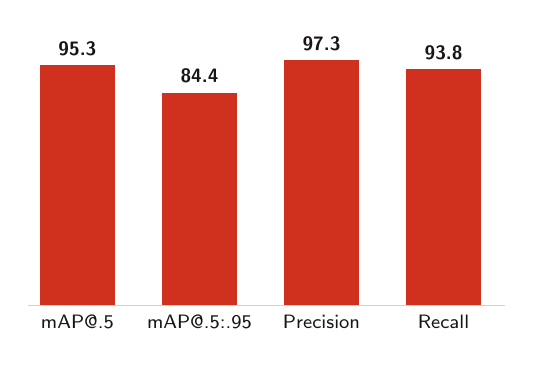
\begin{tikzpicture}[y=0.032cm,x=1cm,font=\scriptsize]
  \foreach \v/\lab/\i in {95.3/{mAP@.5}/0, 84.4/{mAP@.5:.95}/1, 97.3/{Precision}/2, 93.8/{Recall}/3}{
    \fill[mred] (\i*1.55,0) rectangle (\i*1.55+0.95,\v);
    \node[above,text=ink,font=\headfont\bfseries\scriptsize] at (\i*1.55+0.475,\v) {\v};
    \node[below,text=ink,align=center,font=\scriptsize] at (\i*1.55+0.475,0) {\lab};
  }
  \draw[hair] (-0.15,0) -- (5.9,0);
\end{tikzpicture}
\end{tcolorbox}
\end{column}
\begin{column}{0.5\textwidth}
\begin{tcolorbox}[card,height=2.35cm]
{\headfont\bfseries manga-ocr (fine-tuned)}\ {\footnotesize\itshape\textcolor{slate}{OCR tiếng Nhật · test 14.130 mẫu}}\par\vspace{2mm}
{\headfont\bfseries\Large\color{ink}6.1\%}\ {\footnotesize\textcolor{slate}{CER}}\hfill
{\headfont\bfseries\Large\color{ink}93.9\%}\ {\footnotesize\textcolor{slate}{Char-Acc}}\hfill
{\headfont\bfseries\Large\color{ink}67.5\%}\ {\footnotesize\textcolor{slate}{Exact}}
\end{tcolorbox}
\vspace{1.5mm}
\begin{tcolorbox}[creamcard,height=2.35cm]
{\headfont\bfseries Gemini 2.5 Flash}\ {\footnotesize\itshape\textcolor{slate}{Dịch ngữ cảnh · human-in-the-loop}}\par\vspace{2mm}
{\headfont\bfseries\Large\color{mgreen}$\geq$80\%}\ {\footnotesize\textcolor{slate}{hài lòng}}\hfill
{\headfont\bfseries\Large\color{mgreen}2.5 Flash}\ {\footnotesize\textcolor{slate}{Model}}\hfill
{\headfont\bfseries\Large\color{mgreen}768-dim}\ {\footnotesize\textcolor{slate}{Embedding}}
\end{tcolorbox}
\end{column}
\end{columns}
\end{frame}

% ---------------------------------------------------------------------
% SLIDE 14 — TECH STACK
% ---------------------------------------------------------------------
\begin{frame}
\slidehead{III · Công nghệ}{Ngăn xếp công nghệ}
\vspace{0.5mm}\small
\begin{tcbraster}[raster columns=4, raster equal height=rows, raster column skip=2.5mm]
\begin{tcolorbox}[card,colbacktitle=mred,coltitle=white,title={Frontend}]
\begin{itemize}\setlength\itemsep{0.6mm}\item Next.js 16 (App Router)\item React 19 · TypeScript\item Tailwind + Framer Motion\item PWA + offline\end{itemize}\end{tcolorbox}
\begin{tcolorbox}[card,colbacktitle=ink,coltitle=white,title={Backend}]
\begin{itemize}\setlength\itemsep{0.6mm}\item FastAPI · Python 3.11\item Uvicorn / Gunicorn\item SlowAPI rate-limit\item Sentry + OpenTelemetry\end{itemize}\end{tcolorbox}
\begin{tcolorbox}[card,colbacktitle=mgreen,coltitle=white,title={AI / ML}]
\begin{itemize}\setlength\itemsep{0.6mm}\item YOLOv8 (ultralytics)\item manga-ocr (fine-tuned)\item LaMa inpaint\item Gemini 2.5 Flash\end{itemize}\end{tcolorbox}
\begin{tcolorbox}[card,colbacktitle=mblue,coltitle=white,title={Dữ liệu \& Hạ tầng}]
\begin{itemize}\setlength\itemsep{0.6mm}\item Supabase Postgres\item pgvector · pg\_trgm\item Vercel · Render · HF\item GitHub Actions CI\end{itemize}\end{tcolorbox}
\end{tcbraster}
\vspace{1.5mm}{\footnotesize\textcolor{slate}{Mọi thứ chạy trên tier miễn phí/rẻ nhưng vẫn đạt chuẩn production.}}
\end{frame}

% ---------------------------------------------------------------------
% SLIDE 15 — FEATURE HIGHLIGHTS
% ---------------------------------------------------------------------
\begin{frame}
\slidehead{IV · Tính năng nổi bật}{Ngoài lõi dịch — một hệ sinh thái đầy đủ}
\vspace{0.5mm}\footnotesize
\begin{tcbraster}[raster columns=3, raster equal height=rows, raster column skip=2.5mm, raster row skip=2mm]
\begin{tcolorbox}[card]{\numbadge[mred]{1}}\ {\headfont\bfseries Reader nâng cao}\par\textcolor{slate}{Nhiều chế độ đọc, phím tắt, vuốt mobile, từ điển bong bóng, cảnh báo độ tin cậy thấp.}\end{tcolorbox}
\begin{tcolorbox}[card]{\numbadge[ink]{2}}\ {\headfont\bfseries Studio QC}\par\textcolor{slate}{Hiệu đính per-bubble (approve/reject), tìm–thay thế hàng loạt, phản hồi tốt/xấu.}\end{tcolorbox}
\begin{tcolorbox}[card]{\numbadge[mblue]{3}}\ {\headfont\bfseries Thư viện \& chia sẻ}\par\textcolor{slate}{Xuất bản chương công khai, đọc ẩn danh, chia sẻ link TTL + OG image.}\end{tcolorbox}
\begin{tcolorbox}[card]{\numbadge[mgreen]{4}}\ {\headfont\bfseries Cộng đồng}\par\textcolor{slate}{Diễn đàn (mention, đính kèm, vote), bình luận chương, hồ sơ /u/\{username\}.}\end{tcolorbox}
\begin{tcolorbox}[card]{\numbadge[gold]{5}}\ {\headfont\bfseries Gamification (Wibu)}\par\textcolor{slate}{Bookmark, rating, reading list, mục tiêu, XP/level, thành tựu + thông báo.}\end{tcolorbox}
\begin{tcolorbox}[card]{\numbadge[ink2]{6}}\ {\headfont\bfseries Credit \& thanh toán}\par\textcolor{slate}{Free 5/ngày; gói basic/pro/premium; Stripe checkout/webhook; điểm danh streak.}\end{tcolorbox}
\end{tcbraster}
\end{frame}

% ---------------------------------------------------------------------
% SLIDE 16–18 — DEMO (placeholder khung ảnh)
% ---------------------------------------------------------------------
\newcommand{\shotbox}[2]{%
\begin{tcolorbox}[enhanced,sharp corners,colback=cream,colframe=ink,boxrule=1pt,
   borderline={0.6pt}{-1.4pt}{ink,dashed}, halign=center, valign=center, height=4.3cm,
   shadow={0.6mm}{-0.6mm}{0mm}{fill=ink}]
{\Large\textcolor{slate}{\rule{0pt}{0pt}$\square$}}\par\vspace{1mm}
{\headfont\bfseries\footnotesize\textcolor{slate}{CHÈN ẢNH CHỤP MÀN HÌNH}}\par\vspace{1mm}
{\headfont\bfseries\textcolor{mred}{#1}}\par\vspace{1mm}
{\footnotesize\itshape\textcolor{slate}{#2}}
\end{tcolorbox}}

\begin{frame}
\slidehead{IV · Demo · Luồng A}{Trang chủ \& Upload → Dịch}
\begin{columns}
\begin{column}{0.5\textwidth}\shotbox{/ \ (Trang chủ)}{Landing + nền anime động + ‘Tiếp tục đọc’}\end{column}
\begin{column}{0.5\textwidth}\shotbox{/upload}{Kéo-thả trang manga Nhật, chọn cấu hình AI}\end{column}
\end{columns}
\vspace{1.5mm}{\footnotesize{\headfont\bfseries\color{mred}Điểm nhấn khi demo:\ }\textcolor{slate}{đăng nhập \arr\ kéo-thả 1 trang \arr\ pipeline chạy realtime (YOLOv8 \arr\ manga-ocr \arr\ LaMa \arr\ Gemini).}}
\end{frame}

\begin{frame}
\slidehead{IV · Demo · Luồng A}{Reader overlay \& Studio QC}
\begin{columns}
\begin{column}{0.5\textwidth}\shotbox{/reader?page=…}{Bản dịch phủ bong bóng, bật/tắt so sánh}\end{column}
\begin{column}{0.5\textwidth}\shotbox{/studio (QC)}{Hiệu đính per-bubble, tìm–thay thế}\end{column}
\end{columns}
\vspace{1.5mm}{\footnotesize{\headfont\bfseries\color{mred}Điểm nhấn khi demo:\ }\textcolor{slate}{mở Reader xem overlay tiếng Việt; bật/tắt bản gốc; mở từ điển bong bóng; hiệu đính trong Studio.}}
\end{frame}

\begin{frame}
\slidehead{IV · Demo · Luồng B + Q\&A}{Batch cả chương · RAG Q\&A · Thư viện}
\begin{columns}
\begin{column}{0.5\textwidth}\shotbox{/upload (batch) · /qa}{Batch nhiều trang + tiến trình x/N realtime; hỏi–đáp}\end{column}
\begin{column}{0.5\textwidth}\shotbox{/library · /admin}{Thư viện công khai; bảng điều khiển quản trị}\end{column}
\end{columns}
\vspace{1.5mm}{\footnotesize{\headfont\bfseries\color{mred}Điểm nhấn khi demo:\ }\textcolor{slate}{batch cả chương xử lý tuần tự; hỏi AI về nội dung; xuất bản lên thư viện; xem admin dashboard.}}
\end{frame}

% ---------------------------------------------------------------------
% SLIDE 19 — PROCESS
% ---------------------------------------------------------------------
\begin{frame}
\slidehead{IV · Quy trình phát triển}{RUP rút gọn + Scrum theo sprint 2 tuần}
\vspace{0.5mm}\footnotesize
\begin{tcbraster}[raster columns=4, raster equal height=rows, raster column skip=2.4mm]
\begin{tcolorbox}[card]{\kick{Pha 1}}\par{\headfont\bfseries Inception}\par\textcolor{slate}{Vision, kế hoạch, weekly report}\end{tcolorbox}
\begin{tcolorbox}[card]{\kick{Pha 2}}\par{\headfont\bfseries Elaboration}\par\textcolor{slate}{Use case, kiến trúc, UI prototype, test plan}\end{tcolorbox}
\begin{tcolorbox}[card]{\kick{Pha 3}}\par{\headfont\bfseries Construction}\par\textcolor{slate}{Source code, test case, defect, báo cáo}\end{tcolorbox}
\begin{tcolorbox}[creamcard]{\kick{Pha 4}}\par{\headfont\bfseries Transition}\par\textcolor{slate}{Triển khai, demo, nộp bài cuối kỳ}\end{tcolorbox}
\end{tcbraster}
\vspace{2mm}
\begin{columns}[t]
\begin{column}{0.44\textwidth}
\begin{tcolorbox}[darkcard,title={WEEKLY SCRUM},height=3.1cm]\footnotesize\color{white}
\textcolor{mred}{\textbullet}\ Đã làm gì từ tuần trước?\par\vspace{1.2mm}
\textcolor{mred}{\textbullet}\ Đang gặp vướng mắc gì?\par\vspace{1.2mm}
\textcolor{mred}{\textbullet}\ Tuần tới sẽ hoàn thành gì?\par\vspace{1.6mm}
{\itshape\textcolor{softwhite}{Sprint = 2 tuần · PR review trước khi merge · CI xanh mới nộp.}}
\end{tcolorbox}
\end{column}
\begin{column}{0.56\textwidth}
\begin{tcolorbox}[card,title={\textcolor{mred}{VAI TRÒ THEO RUP (mẫu)}},height=3.1cm]\footnotesize
\begin{tabular}{@{}p{3cm}p{5cm}@{}}
{\headfont\bfseries Team Lead / PM} & \textcolor{slate}{Kế hoạch, phân công, weekly report}\\
{\headfont\bfseries Business Analyst} & \textcolor{slate}{Thu thập \& rà soát yêu cầu}\\
{\headfont\bfseries Designer} & \textcolor{slate}{Kiến trúc, UI, tài liệu SAD}\\
{\headfont\bfseries\color{mred}Implementer ×3} & \textcolor{slate}{Source code, unit test, review}\\
{\headfont\bfseries Tester} & \textcolor{slate}{Test plan, test case, system test}\\
\end{tabular}
\end{tcolorbox}
\end{column}
\end{columns}
\end{frame}

% ---------------------------------------------------------------------
% SLIDE 19B — TEAM ORGANIZATION & RESPONSIBILITIES
% ---------------------------------------------------------------------
\begin{frame}
\slidehead{IV · Tổ chức nhóm}{Cơ cấu nhóm \& phân công công việc}
\vspace{0.5mm}
{\footnotesize{\headfont\bfseries Nhóm 6 thành viên · mô hình phẳng (flat team) —\ }\textcolor{slate}{không cấp bậc cứng nhắc; mọi quyết định kỹ thuật quan trọng được thảo luận tập thể.}}\par\vspace{2mm}
\renewcommand{\arraystretch}{1.35}
\arrayrulecolor{hair}
\scriptsize
\begin{tabular}{|>{\raggedright\arraybackslash}p{1.15cm}|>{\raggedright\arraybackslash}p{2.5cm}|>{\raggedright\arraybackslash}p{2.9cm}|>{\raggedright\arraybackslash}p{5.7cm}|}
\hline
\rowcolor{ink}
{\color{white}\headfont\bfseries MSSV} & {\color{white}\headfont\bfseries Họ và tên} & {\color{white}\headfont\bfseries Vai trò} & {\color{white}\headfont\bfseries Trách nhiệm chính}\\
\hline
\textcolor{slate}{23122041} & {\headfont\bfseries Đào Sỹ Duy Minh} & {\headfont\bfseries\color{mred}Project Manager \& AI/ML} & \textcolor{ink2}{Quản lý tiến độ, điều phối nhóm · Fine-tune OCR cho manga tiếng Nhật · Prompt engineering cho dịch LLM}\\
\hline
\rowcolor{cream}
\textcolor{slate}{23122002} & {\headfont\bfseries Nguyễn Đình Hà Dương} & {\headfont\bfseries\color{mred}AI/ML Engineer (OCR)} & \textcolor{ink2}{Chuẩn bị \& xử lý dataset manga · Hỗ trợ fine-tune OCR · Đánh giá accuracy, phân tích lỗi}\\
\hline
\textcolor{slate}{23122039} & {\headfont\bfseries Huỳnh Trung Kiệt} & {\headfont\bfseries\color{ink}Backend Developer} & \textcolor{ink2}{FastAPI backend · Thiết kế cơ sở dữ liệu · Tích hợp pipeline OCR/dịch vào server}\\
\hline
\rowcolor{cream}
\textcolor{slate}{23122030} & {\headfont\bfseries Phạm Phú Hòa} & {\headfont\bfseries\color{mgreen}AI/ML Engineer (RAG)} & \textcolor{ink2}{Tích hợp LLM (Gemini) · Vector database (pgvector) · Pipeline hỏi–đáp RAG}\\
\hline
\textcolor{slate}{23122044} & {\headfont\bfseries Trần Chí Nguyên} & {\headfont\bfseries\color{mblue}Frontend Developer} & \textcolor{ink2}{Giao diện Next.js/React (UI-UX) · Upload \& Reader · Màn hình hỏi–đáp Q\&A}\\
\hline
\rowcolor{cream}
\textcolor{slate}{23122048} & {\headfont\bfseries Nguyễn Lâm Phú Quý} & {\headfont\bfseries\color{gold}QA \& Business Analyst} & \textcolor{ink2}{Tài liệu (SDP, Vision, Use case) · Test case \& test plan · UAT, kiểm thử end-to-end}\\
\hline
\end{tabular}
\end{frame}

% ---------------------------------------------------------------------
% SLIDE 20 — TESTING & CI  (Katalon = PA5)
% ---------------------------------------------------------------------
\begin{frame}
\slidehead{IV · Kiểm thử \& CI/CD}{Chất lượng được kiểm thử \& tự động hoá}
\vspace{0.5mm}
\begin{columns}[t]
\begin{column}{0.5\textwidth}\scriptsize
\begin{tcolorbox}[card,title={Tầng kiểm thử},height=5.7cm]
{\numbadge[mred]{1}}\ {\headfont\bfseries Katalon Studio}\ {\color{mred}\bfseries · PA5}\par
\textcolor{slate}{UI tự động: UC01 Upload–Dịch \& UC02 Đọc overlay · $\geq$2 scenario/UC · Pass/Fail.}\par\vspace{1.4mm}
{\numbadge[gold]{2}}\ {\headfont\bfseries Unit / Component}\par\textcolor{slate}{Vitest + React Testing Library (frontend).}\par\vspace{1.4mm}
{\numbadge[ink]{3}}\ {\headfont\bfseries Backend}\par\textcolor{slate}{pytest + respx (mock Supabase/Gemini).}\par\vspace{1.4mm}
{\numbadge[mblue]{4}}\ {\headfont\bfseries E2E}\par\textcolor{slate}{Playwright: auth, home, protected, mobile, forum, edge-cases.}\par\vspace{1.4mm}
{\numbadge[mgreen]{5}}\ {\headfont\bfseries Tĩnh}\par\textcolor{slate}{tsc --noEmit · ESLint · Python type hints.}
\end{tcolorbox}
\end{column}
\begin{column}{0.5\textwidth}\footnotesize
\begin{tcolorbox}[darkcard,title={GITHUB ACTIONS · 5 JOB SONG SONG},height=5.7cm]\color{white}
\textcolor{mgreen}{\checkmark}\ Typecheck (tsc)\par\vspace{2.4mm}
\textcolor{mgreen}{\checkmark}\ Lint (ESLint)\par\vspace{2.4mm}
\textcolor{mgreen}{\checkmark}\ Production build\par\vspace{2.4mm}
\textcolor{mgreen}{\checkmark}\ Playwright E2E\par\vspace{2.4mm}
\textcolor{mgreen}{\checkmark}\ Backend pytest\par\vspace{3mm}
{\itshape\textcolor{softwhite}{Mọi PR phải review + CI xanh trước khi merge vào main.}}
\end{tcolorbox}
\end{column}
\end{columns}
\end{frame}

% ---------------------------------------------------------------------
% SLIDE 21 — SECURITY
% ---------------------------------------------------------------------
\begin{frame}
\slidehead{IV · Bảo mật}{Phòng thủ nhiều lớp}
\vspace{0.5mm}\footnotesize
\begin{tcbraster}[raster columns=3, raster equal height=rows, raster column skip=2.5mm, raster row skip=2mm]
\begin{tcolorbox}[card]{\headfont\bfseries\color{ink}Xác thực}\par\textcolor{slate}{Cookie HttpOnly (không lộ token cho JS); auto-refresh; Google OAuth.}\end{tcolorbox}
\begin{tcolorbox}[creamcard]{\headfont\bfseries\color{ink}Phân quyền}\par\textcolor{slate}{RBAC user/admin ở API + RLS trên mọi bảng dữ liệu người dùng.}\end{tcolorbox}
\begin{tcolorbox}[card]{\headfont\bfseries\color{ink}Chống lạm dụng}\par\textcolor{slate}{Rate-limit (SlowAPI) theo endpoint; captcha Turnstile ở đăng ký / quên MK.}\end{tcolorbox}
\begin{tcolorbox}[creamcard]{\headfont\bfseries\color{ink}Header \& CSP}\par\textcolor{slate}{Security headers + CSP chặt trên mọi response, kể cả /docs.}\end{tcolorbox}
\begin{tcolorbox}[card]{\headfont\bfseries\color{ink}Kiểm tra upload}\par\textcolor{slate}{Pillow verify() chống giả mạo MIME; chỉ nhận JPEG/PNG/WebP thật.}\end{tcolorbox}
\begin{tcolorbox}[creamcard]{\headfont\bfseries\color{ink}Chống SSRF}\par\textcolor{slate}{scraper chỉ nhận domain trong allowlist khi nhập từ nguồn ngoài.}\end{tcolorbox}
\end{tcbraster}
\end{frame}

% ---------------------------------------------------------------------
% SLIDE 22 — DEPLOYMENT
% ---------------------------------------------------------------------
\begin{frame}
\slidehead{IV · Triển khai}{Bốn nền tảng, tự động deploy từ main}
\vspace{0.5mm}\footnotesize
\begin{tcbraster}[raster columns=4, raster equal height=rows, raster column skip=2.5mm]
\begin{tcolorbox}[card,colbacktitle=mred,coltitle=white,title={Frontend}]{\headfont\bfseries\large Vercel}\par{\color{mred}\bfseries Global CDN}\par\vspace{1mm}\textcolor{slate}{Auto-deploy khi push main}\end{tcolorbox}
\begin{tcolorbox}[card,colbacktitle=ink,coltitle=white,title={Backend API}]{\headfont\bfseries\large Render}\par{\color{ink}\bfseries Singapore · Docker}\par\vspace{1mm}\textcolor{slate}{render.yaml · free tier 512MB}\end{tcolorbox}
\begin{tcolorbox}[card,colbacktitle=mgreen,coltitle=white,title={AI Module}]{\headfont\bfseries\large HuggingFace}\par{\color{mgreen}\bfseries Spaces · ~4GB}\par\vspace{1mm}\textcolor{slate}{Deploy Docker thủ công}\end{tcolorbox}
\begin{tcolorbox}[card,colbacktitle=mblue,coltitle=white,title={DB + Storage}]{\headfont\bfseries\large Supabase}\par{\color{mblue}\bfseries AWS us-east-1}\par\vspace{1mm}\textcolor{slate}{Postgres + pgvector + Auth}\end{tcolorbox}
\end{tcbraster}
\vspace{2mm}
\begin{tcolorbox}[creamcard]\small
{\headfont\bfseries\color{mred}Vận hành:\ }keep-alive ping chống ngủ (Render/HF) · health check /health \& /health/deep · Sentry + OpenTelemetry giám sát · Supabase PITR backup 7 ngày.
\end{tcolorbox}
\end{frame}

% ---------------------------------------------------------------------
% SLIDE 23 — LIMITATIONS
% ---------------------------------------------------------------------
\begin{frame}
\slidehead{V · Nhìn thẳng vào hạn chế}{Hạn chế \& lỗi đã biết}
\vspace{0.5mm}
\begin{columns}[t]
\begin{column}{0.5\textwidth}\scriptsize
\begin{tcolorbox}[card]{\headfont\bfseries\color{mred}Cold start}\par\textcolor{slate}{Render free \& HF Spaces ngủ khi rảnh \arr\ lần đầu chậm 15–60s (đã có keep-alive).}\end{tcolorbox}\vspace{1.2mm}
\begin{tcolorbox}[card]{\headfont\bfseries\color{mred}Quota Gemini}\par\textcolor{slate}{Free tier giới hạn RPD \arr\ xoay vòng key + throttle + cache; cao điểm vẫn có thể bị giới hạn.}\end{tcolorbox}\vspace{1.2mm}
\begin{tcolorbox}[card]{\headfont\bfseries\color{mred}OCR chữ hiệu ứng (SFX)}\par\textcolor{slate}{Chữ viết tay / hiệu ứng độ chính xác giảm; bong bóng SFX có thể bị bỏ qua.}\end{tcolorbox}\vspace{1.2mm}
\begin{tcolorbox}[card]{\headfont\bfseries\color{mred}Bố cục chữ Việt dài}\par\textcolor{slate}{Bong bóng nhỏ phải thu nhỏ cỡ chữ hoặc cắt bớt (có tooltip đầy đủ).}\end{tcolorbox}
\end{column}
\begin{column}{0.5\textwidth}
\begin{tcolorbox}[darkcard,title={LỖI ĐÃ BIẾT (đang xử lý)},height=6.3cm]\footnotesize\color{white}
\textcolor{mred}{\textbullet}\ Token phiên hết hạn giữa chừng \arr\ đôi khi cần tải lại trang (đang hoàn thiện auto-refresh).\par\vspace{2.6mm}
\textcolor{mred}{\textbullet}\ WebSocket mất gói khi mạng chập chờn \arr\ fallback polling, tiến trình có thể ‘nhảy’ \%.\par\vspace{2.6mm}
\textcolor{mred}{\textbullet}\ Signed URL ảnh có thể hết hạn với phiên đọc rất dài \arr\ đã thêm retry tải ảnh.\par\vspace{2.6mm}
\textcolor{mred}{\textbullet}\ Thiết bị mobile cũ: nền anime động có thể tụt FPS (tắt được trong cài đặt).
\end{tcolorbox}
\end{column}
\end{columns}
\end{frame}

% ---------------------------------------------------------------------
% SLIDE 24 — FUTURE WORK
% ---------------------------------------------------------------------
\begin{frame}
\slidehead{V · Hướng phát triển}{Roadmap tiếp theo}
\vspace{0.5mm}\footnotesize
\begin{tcbraster}[raster columns=3, raster equal height=rows, raster column skip=2.5mm, raster row skip=2mm]
\begin{tcolorbox}[card]{\headfont\bfseries\color{mred}\arr\ OCR \& dịch tốt hơn}\par\textcolor{slate}{Fine-tune thêm cho SFX/chữ viết tay; hỗ trợ thêm cặp ngôn ngữ (Hàn, Anh).}\end{tcolorbox}
\begin{tcolorbox}[creamcard]{\headfont\bfseries\color{mred}\arr\ Sắp xếp bong bóng RTL}\par\textcolor{slate}{Cải thiện thứ tự đọc phải-sang-trái cho bố cục phức tạp.}\end{tcolorbox}
\begin{tcolorbox}[card]{\headfont\bfseries\color{mred}\arr\ Nâng độ sẵn sàng}\par\textcolor{slate}{Chuyển tier trả phí giảm cold start; hàng đợi tác vụ chuyên dụng.}\end{tcolorbox}
\begin{tcolorbox}[creamcard]{\headfont\bfseries\color{mred}\arr\ Cá nhân hoá}\par\textcolor{slate}{Gợi ý truyện theo lịch sử đọc; cải thiện RAG đa-trang / cả series.}\end{tcolorbox}
\begin{tcolorbox}[card]{\headfont\bfseries\color{mred}\arr\ Kiểm duyệt \& bản quyền}\par\textcolor{slate}{Công cụ chống vi phạm bản quyền, quy trình DMCA rõ ràng.}\end{tcolorbox}
\begin{tcolorbox}[creamcard]{\headfont\bfseries\color{mred}\arr\ Ứng dụng di động}\par\textcolor{slate}{Đóng gói PWA thành app; đọc offline mượt hơn.}\end{tcolorbox}
\end{tcbraster}
\end{frame}

% ---------------------------------------------------------------------
% SLIDE 25 — CONCLUSION (dark)
% ---------------------------------------------------------------------
{\setbeamercolor{background canvas}{bg=ink}
\begin{frame}[plain]
\begin{tikzpicture}[remember picture,overlay]
  \fill[mred] (current page.north west) rectangle ++(0.22,-\paperheight);
\end{tikzpicture}
\hspace{0.5cm}\begin{minipage}{0.92\paperwidth}
\kickg{V · Kết luận}\par\vspace{1.5mm}
{\headfont\bfseries\huge\textcolor{white}{Một sản phẩm AI hoàn chỉnh, chạy thật.}}\par\vspace{4mm}
\begin{tcbraster}[raster columns=4, raster equal height=rows, raster column skip=3mm]
\begin{tcolorbox}[enhanced,sharp corners,colback=ink2,colframe=ink2,coltext=white,boxrule=0pt,halign=flush left]{\headfont\bfseries\huge\color{mred}3}\par{\footnotesize\color{softwhite}dịch vụ triển khai độc lập}\end{tcolorbox}
\begin{tcolorbox}[enhanced,sharp corners,colback=ink2,colframe=ink2,coltext=white,boxrule=0pt,halign=flush left]{\headfont\bfseries\huge\color{gold}95.3\%}\par{\footnotesize\color{softwhite}mAP@0.5 phát hiện bong bóng}\end{tcolorbox}
\begin{tcolorbox}[enhanced,sharp corners,colback=ink2,colframe=ink2,coltext=white,boxrule=0pt,halign=flush left]{\headfont\bfseries\huge\color{gold}6.1\%}\par{\footnotesize\color{softwhite}CER OCR tiếng Nhật}\end{tcolorbox}
\begin{tcolorbox}[enhanced,sharp corners,colback=ink2,colframe=ink2,coltext=white,boxrule=0pt,halign=flush left]{\headfont\bfseries\huge\color{white}9+}\par{\footnotesize\color{softwhite}nhóm yêu cầu chức năng}\end{tcolorbox}
\end{tcbraster}
\vspace{3mm}
\begin{tcolorbox}[enhanced,sharp corners,colback=ink2,colframe=ink2,coltext=white,boxrule=0pt,fonttitle=\headfont\bfseries\color{gold},title={ĐIỀU ĐẠT ĐƯỢC}]\small\color{white}
\textcolor{gold}{\textbullet}\ Pipeline AI end-to-end: phát hiện \arr\ OCR \arr\ xoá nền \arr\ dịch ngữ cảnh \arr\ RAG Q\&A.\par\vspace{1.6mm}
\textcolor{gold}{\textbullet}\ Kỹ thuật production: microservice, WebSocket, bảo mật nhiều lớp, CI 5 job, giám sát.\par\vspace{1.6mm}
\textcolor{gold}{\textbullet}\ Áp dụng quy trình CNPM: RUP rút gọn + Scrum, tài liệu SAD/SRS/SDP đồng bộ code thật.
\end{tcolorbox}
\end{minipage}
\end{frame}}

% ---------------------------------------------------------------------
% SLIDE 26 — THANK YOU / Q&A (dark)
% ---------------------------------------------------------------------
{\setbeamercolor{background canvas}{bg=ink}
\begin{frame}[plain]
\begin{tikzpicture}[remember picture,overlay]
  \fill[gold] ($(current page.south east)+(-1.9,1.0)$) rectangle ++(0.9,0.9);
  \fill[mred] ($(current page.south east)+(-1.55,0.65)$) rectangle ++(0.9,0.9);
  \fill[mred] ($(current page.north east)+(-1.78,-0.6)$) rectangle ++(1.4,-1.4);
  \fill[white] ($(current page.north east)+(-1.88,-0.5)$) rectangle ++(1.4,-1.4);
  \node[anchor=north east,inner sep=0] at ($(current page.north east)+(-0.6,-0.62)$)
     {
\includegraphics[width=1.16cm]{assets/hcmus_logo.png}};
\end{tikzpicture}
\vspace{1.4cm}
\hspace{0.6cm}\begin{minipage}{0.9\paperwidth}
\kickg{Cảm ơn Thầy \& các bạn đã lắng nghe}\par\vspace{2mm}
{\headfont\bfseries\fontsize{40}{44}\selectfont\textcolor{white}{Câu hỏi \& Thảo luận}}\par\vspace{2.5mm}
{\color{mred}\rule{6cm}{1.6pt}}\par\vspace{2mm}
{\headfont\bfseries\Large\textcolor{mred}{StoryLens}}\par\vspace{4mm}
\footnotesize
\begin{tabular}{@{}p{3cm}l@{}}
{\color{gold}\headfont\bfseries WEB} & {\color{white}storylens-api.onrender.com}\\[1mm]
{\color{gold}\headfont\bfseries AI MODULE} & {\color{white}huynhtrungkiet09032005-ai-storylen.hf.space}\\[1mm]
{\color{gold}\headfont\bfseries TÀI KHOẢN DEMO} & {\color{white}demo.pa3@storylens.app}\\[1mm]
{\color{gold}\headfont\bfseries NHÓM} & {\color{white}Nhóm 1 — CSC10011 · GVHD: GS.TS Nguyễn Văn Vũ}\\
\end{tabular}
\end{minipage}
\end{frame}}

\end{document}
